% 9 variables in here:
% h_1 = 10.0, h_2 = 10.0, h_3 = 10.0, ux_1 = 0.0, ux_2 = 0.0, ux_3 = 0.0, uy_1 = 0.0, uy_2 = 0.0, uy_3 = 0.0
\begin{figure}[h!]
\centering
  \subfigure[Height values are 10, $h_1$ ranges from 8 to 12. All impulses are 0.] {
    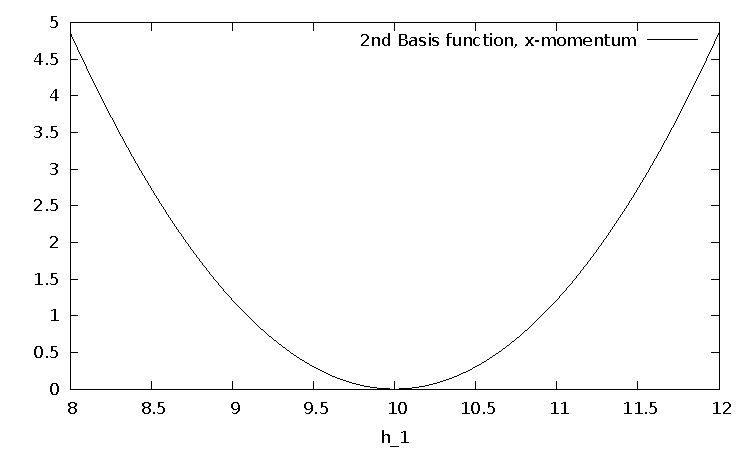
\includegraphics[scale=\zoomfactor]{{{magnitude_10_default/y_10.0_10.0_0.0_0.0_0.0_0.0_0.0_0.0f02}}}
  }
  \subfigure[Height values are 1000, $h_1$ ranges from 998 to 1002. All impulses are 0.] {
    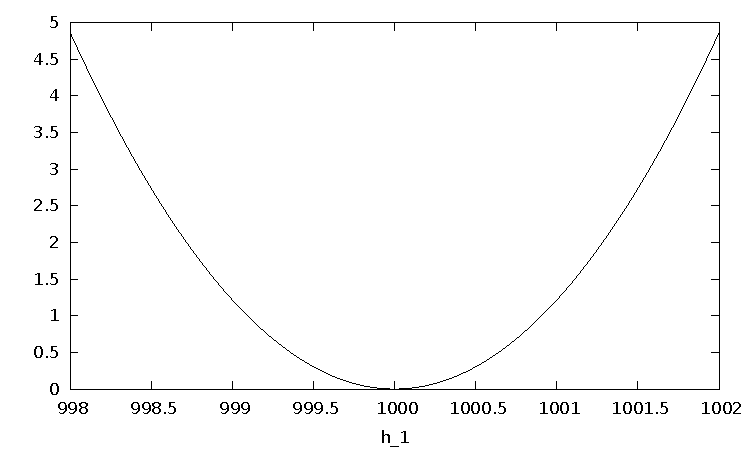
\includegraphics[scale=\zoomfactor]{{{magnitude_1000_default/y_1000.0_1000.0_0.0_0.0_0.0_0.0_0.0_0.0f02}}}
  }
\caption{Comparison of different orders of magnitudes for standard values.}
\label{fig:magnitude_10_default}
\end{figure}

%%% Local Variables:
%%% TeX-master: "../results.tex"
%%% End:
% 9 variables in here:
% h_1 = 10.0, h_2 = 10.0, h_3 = 10.0, ux_1 = 0.0, ux_2 = 0.0, ux_3 = 0.0, uy_1 = 0.0, uy_2 = 0.0, uy_3 = 0.0
\begin{figure}[h!]
\centering
  \subfigure[] {
    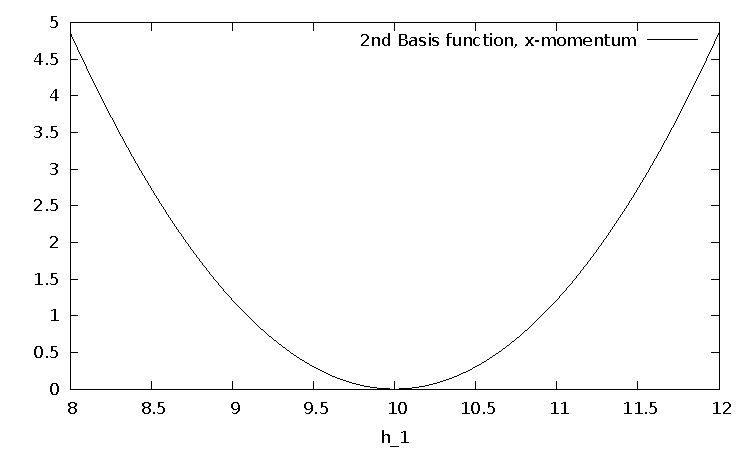
\includegraphics[scale=\zoomfactor]{{{magnitude_10_default/y_10.0_10.0_0.0_0.0_0.0_0.0_0.0_0.0f02}}}
  }
\caption{}
\label{fig:magnitude_10_default}
\end{figure}

%%% Local Variables:
%%% TeX-master: "../results.tex"
%%% End:
% 9 variables in here:
% h_1 = 10.0, h_2 = 10.0, h_3 = 10.0, ux_1 = 0.0, ux_2 = 0.0, ux_3 = 0.0, uy_1 = 0.0, uy_2 = 0.0, uy_3 = 0.0
\begin{figure}[h!]
\centering
  \subfigure[] {
    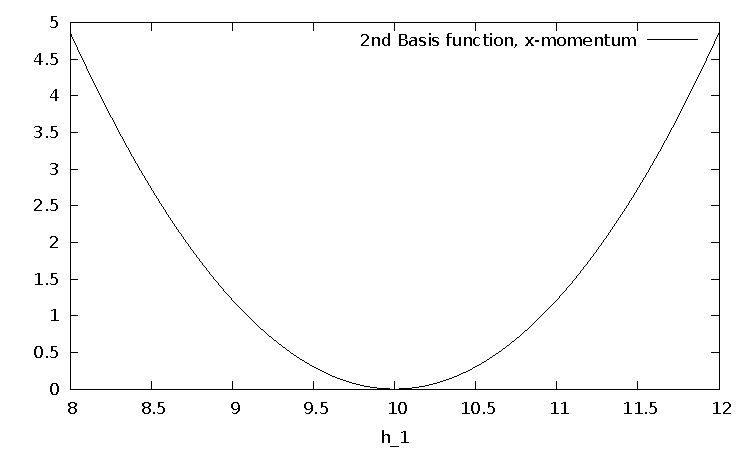
\includegraphics[scale=\zoomfactor]{{{magnitude_10_default/y_10.0_10.0_0.0_0.0_0.0_0.0_0.0_0.0f02}}}
  }
\caption{}
\label{fig:magnitude_10_default}
\end{figure}

%%% Local Variables:
%%% TeX-master: "../results.tex"
%%% End:
